% ==================================================================
% 4 RESULTADOS
% ==================================================================

\chapter{RESULTADOS}

Este capítulo apresenta os resultados empíricos da comparação entre as três estratégias de alocação de ativos implementadas: Equal Weight, otimização de Markowitz e Risk Parity. A análise baseia-se em dados reais do mercado acionário brasileiro durante o período de teste 2018-2019, utilizando carteiras construídas com informações disponíveis apenas até dezembro de 2017.

Os resultados são organizados em cinco seções principais: (1) performance geral das estratégias, (2) evolução temporal dos retornos, (3) análise de risco através de drawdowns, (4) validação estatística das diferenças observadas, e (5) características de implementação das carteiras. Esta estrutura permite análise abrangente tanto da eficácia relativa das estratégias quanto de sua viabilidade prática.

\section{PERFORMANCE GERAL DAS ESTRATÉGIAS}

A Tabela~\ref{tab:performance_completa} apresenta as métricas de performance das três estratégias durante o período de análise. Os resultados mostram diferenças substanciais entre as abordagens, tanto em termos de retorno quanto de características de risco.

\begin{table}[H]
\centering
\caption{Performance das estratégias de alocação (2018-2019)}
\label{tab:performance_completa}
\begin{tabular}{lrrrrrrrrr}
\toprule
Estratégia & Retorno Anual (\%) & Volatilidade (\%) & Sharpe Ratio & Sortino Ratio & Max Drawdown (\%) & Retorno Total (\%) & Prob. Ganho (\%) & Skewness & Kurtosis \\
\midrule
Equal Weight & 29.84 & 19.72 & 1.197 & 1.105 & -18.88 & 73.85 & 70.83 & -0.635 & 1.446 \\
Markowitz & 42.45 & 19.49 & 1.858 & 2.385 & -14.61 & 122.53 & 70.83 & -0.300 & -0.521 \\
Risk Parity & 28.75 & 18.62 & 1.209 & 1.256 & -18.19 & 70.84 & 70.83 & -0.740 & 1.426 \\
\bottomrule
\end{tabular}
\footnotesize
Fonte: Elaboração própria. Dados: Economática. Período: jan/2018 - dez/2019.
\end{table}

A estratégia Markowitz apresentou o maior Sharpe Ratio (1,858), superando significativamente Risk Parity (1,209) e Equal Weight (1,197), indicando melhor relação risco-retorno ajustada. Em termos de retorno absoluto, Markowitz obteve o maior retorno anualizado (42,45\%), seguido por Equal Weight (29,84\%) e Risk Parity (28,75\%).

A análise de risco revela padrões interessantes. Risk Parity apresentou a menor volatilidade anualizada (18,62\%), demonstrando eficácia na diversificação de risco. O maximum drawdown, métrica crucial para avaliação de risco de cauda, foi mais favorável para Markowitz (-14,61\%) comparado a Risk Parity (-18,19\%) e Equal Weight (-18,88\%).

As métricas de assimetria (skewness) e curtose (kurtosis) indicam características distributivas distintas. Markowitz apresentou skewness menos negativa (-0,300), sugerindo distribuição de retornos mais equilibrada, enquanto Equal Weight e Risk Parity mostraram skewness mais negativas (-0,635 e -0,740 respectivamente) e curtose positiva, indicando caudas mais pesadas.

\section{EVOLUÇÃO TEMPORAL DOS RETORNOS}

A Figura~\ref{fig:retornos_acumulados} ilustra a evolução dos retornos acumulados das três estratégias ao longo do período de análise, destacando eventos macroeconômicos relevantes que impactaram o mercado brasileiro.

\begin{figure}[H]
\centering
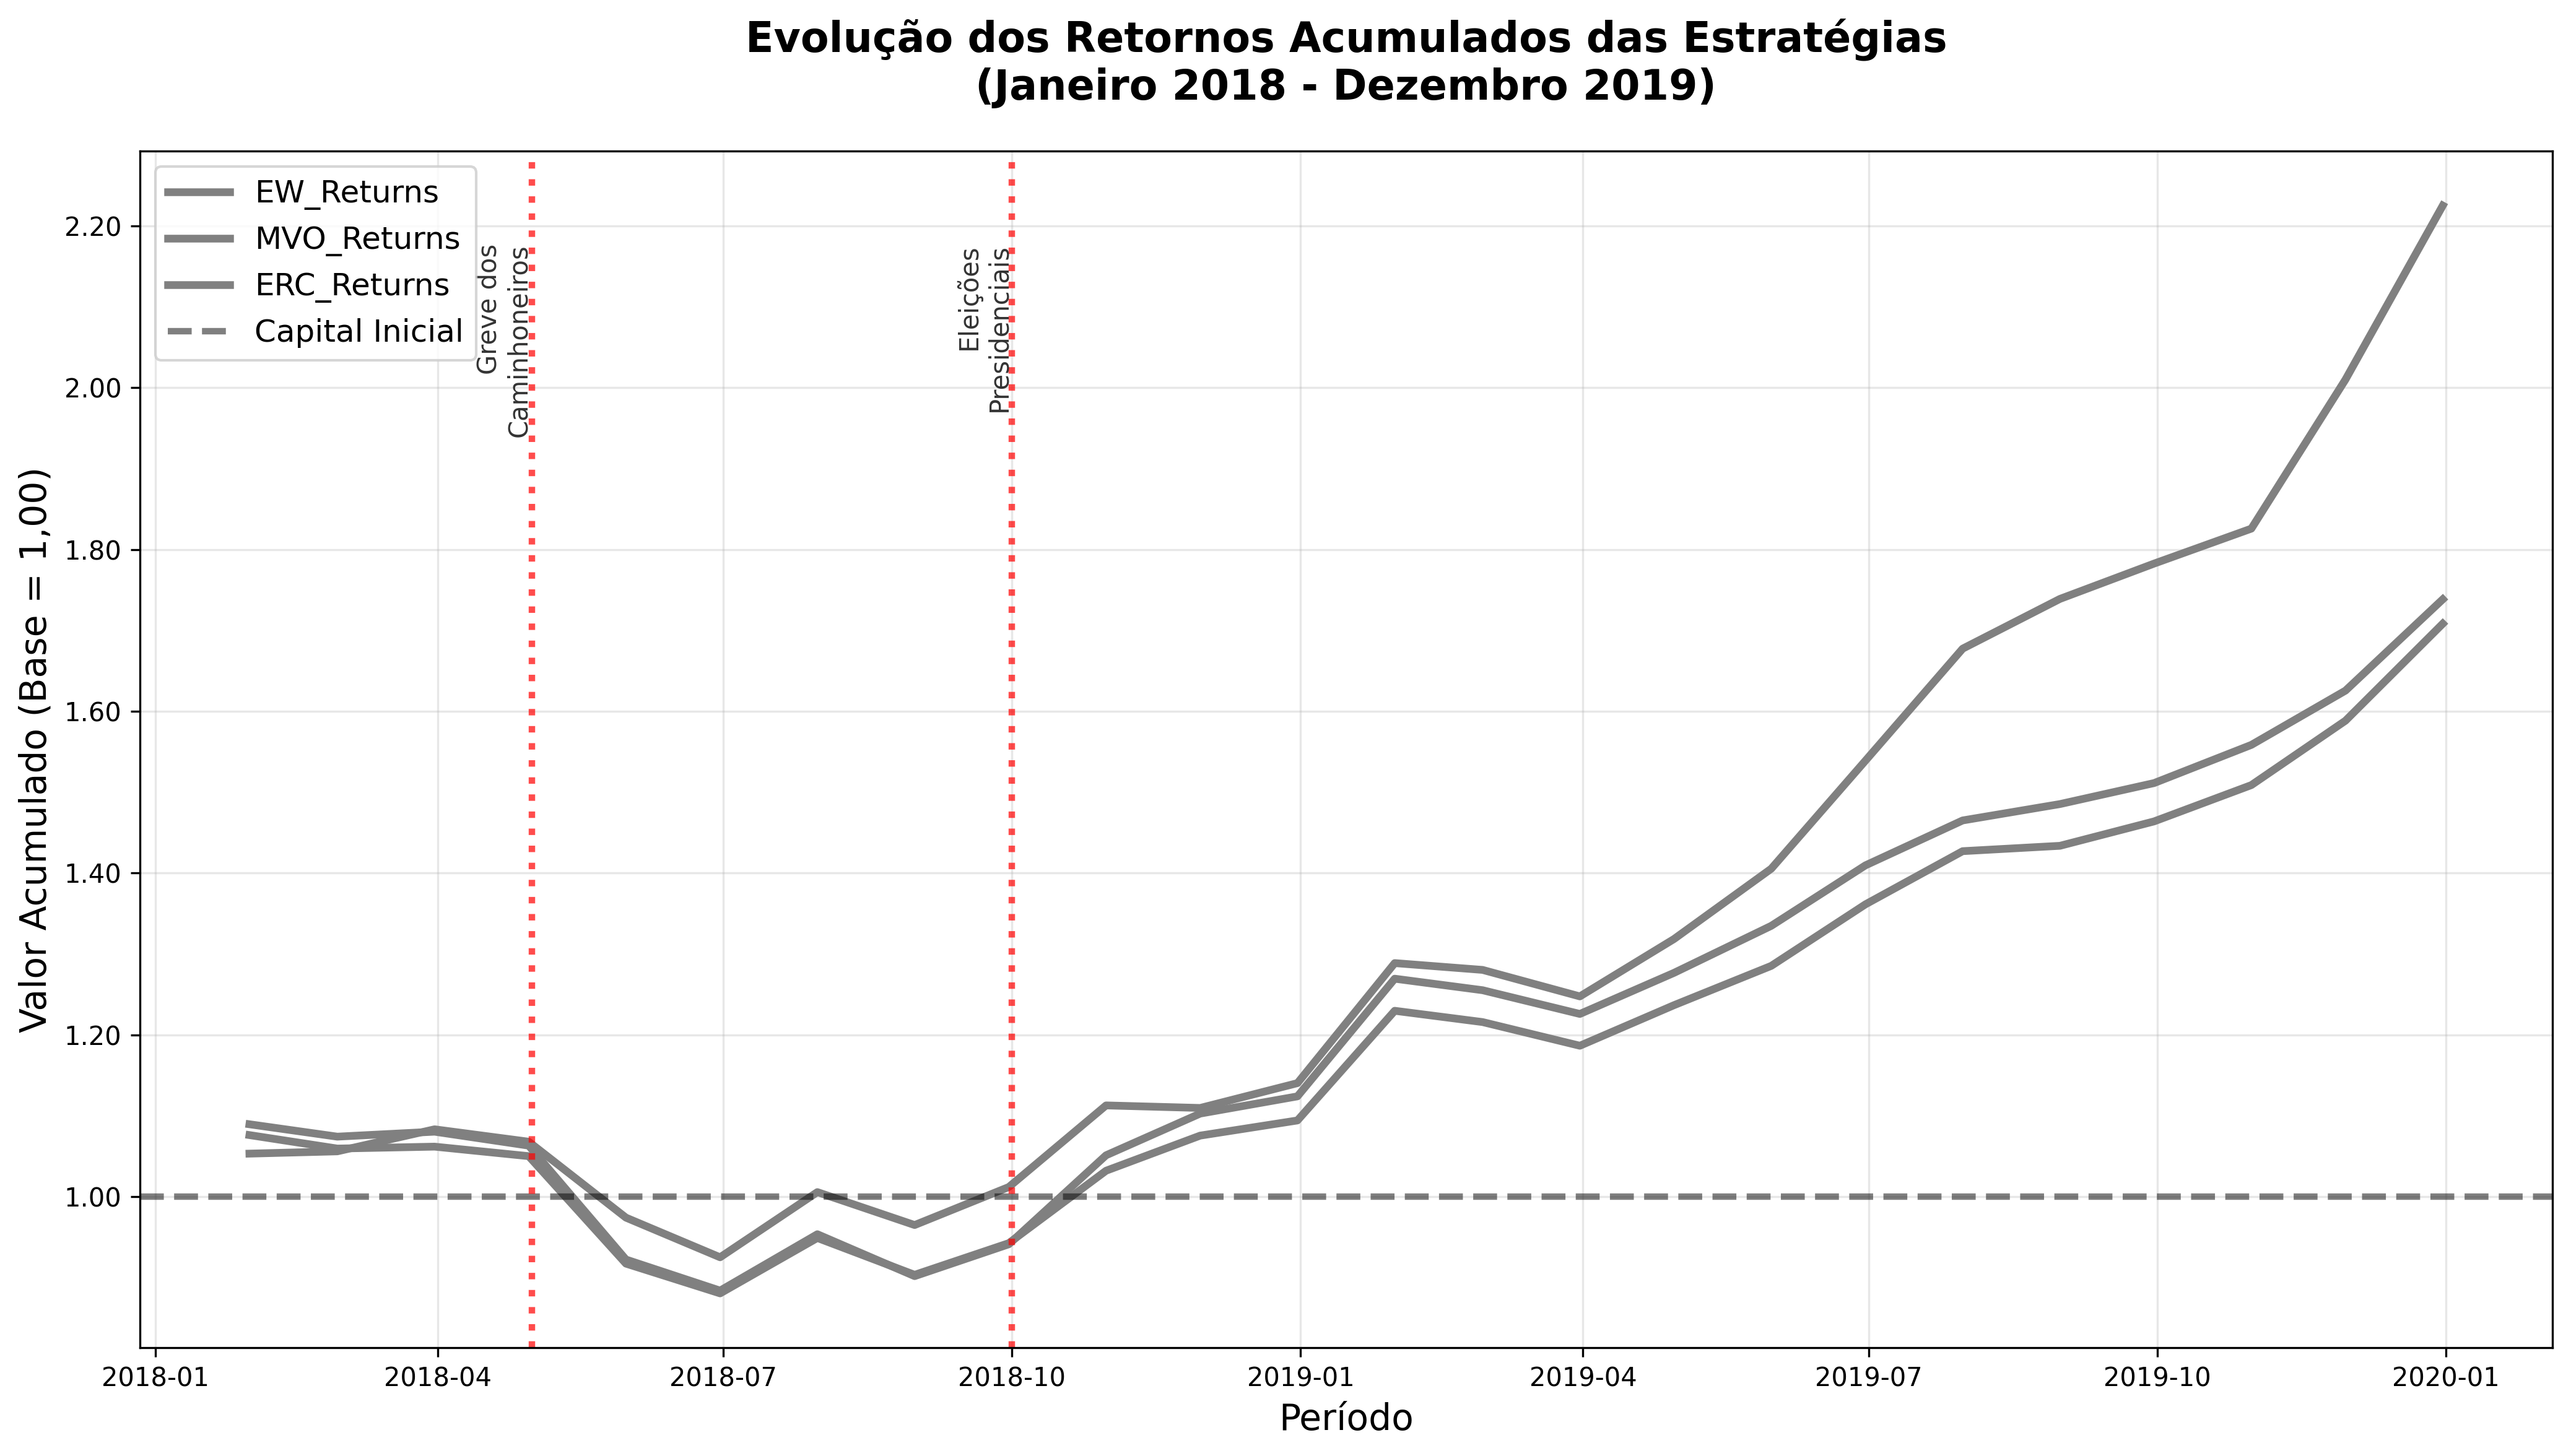
\includegraphics[width=\textwidth]{figures/retornos_acumulados_essencial.png}
\caption{Evolução dos retornos acumulados das estratégias (2018-2019)}
\label{fig:retornos_acumulados}
\footnotesize
Fonte: Elaboração própria. Base = 1,00 em janeiro de 2018.
\end{figure}

A análise temporal revela três fases distintas de performance. No primeiro trimestre de 2018, todas as estratégias apresentaram performance similar, com ligeira vantagem para Markowitz. Durante a greve dos caminhoneiros (maio 2018), observa-se divergência significativa: Markowitz manteve trajetória ascendente mais robusta, Equal Weight apresentou crescimento moderado, enquanto Risk Parity mostrou maior estabilidade mas menor crescimento.

O período eleitoral (setembro-outubro 2018) marca ponto de inflexão importante. Markowitz demonstrou capacidade superior de capturar oportunidades durante a incerteza política, consolidando sua vantagem de performance. Risk Parity manteve trajetória mais estável mas com menor crescimento, enquanto Equal Weight apresentou comportamento intermediário. Esta diferença de comportamento reflete as características intrínsecas de cada abordagem: Markowitz, por sua otimização, conseguiu identificar combinações mais eficientes durante períodos de volatilidade.

O ano de 2019 consolidou a vantagem de Markowitz em termos de retorno absoluto, atingindo retorno acumulado total de 122,53\% ao final do período. Equal Weight alcançou 73,85\%, demonstrando crescimento sólido, enquanto Risk Parity apresentou retorno total de 70,84\%, refletindo sua abordagem mais conservadora e focada no controle de risco.

\section{ANÁLISE DE RISCO ATRAVÉS DE DRAWDOWNS}

A Figura~\ref{fig:drawdowns} apresenta a evolução dos drawdowns das estratégias, oferecendo perspectiva crucial sobre o comportamento em períodos de estresse e a velocidade de recuperação após perdas.

\begin{figure}[H]
\centering
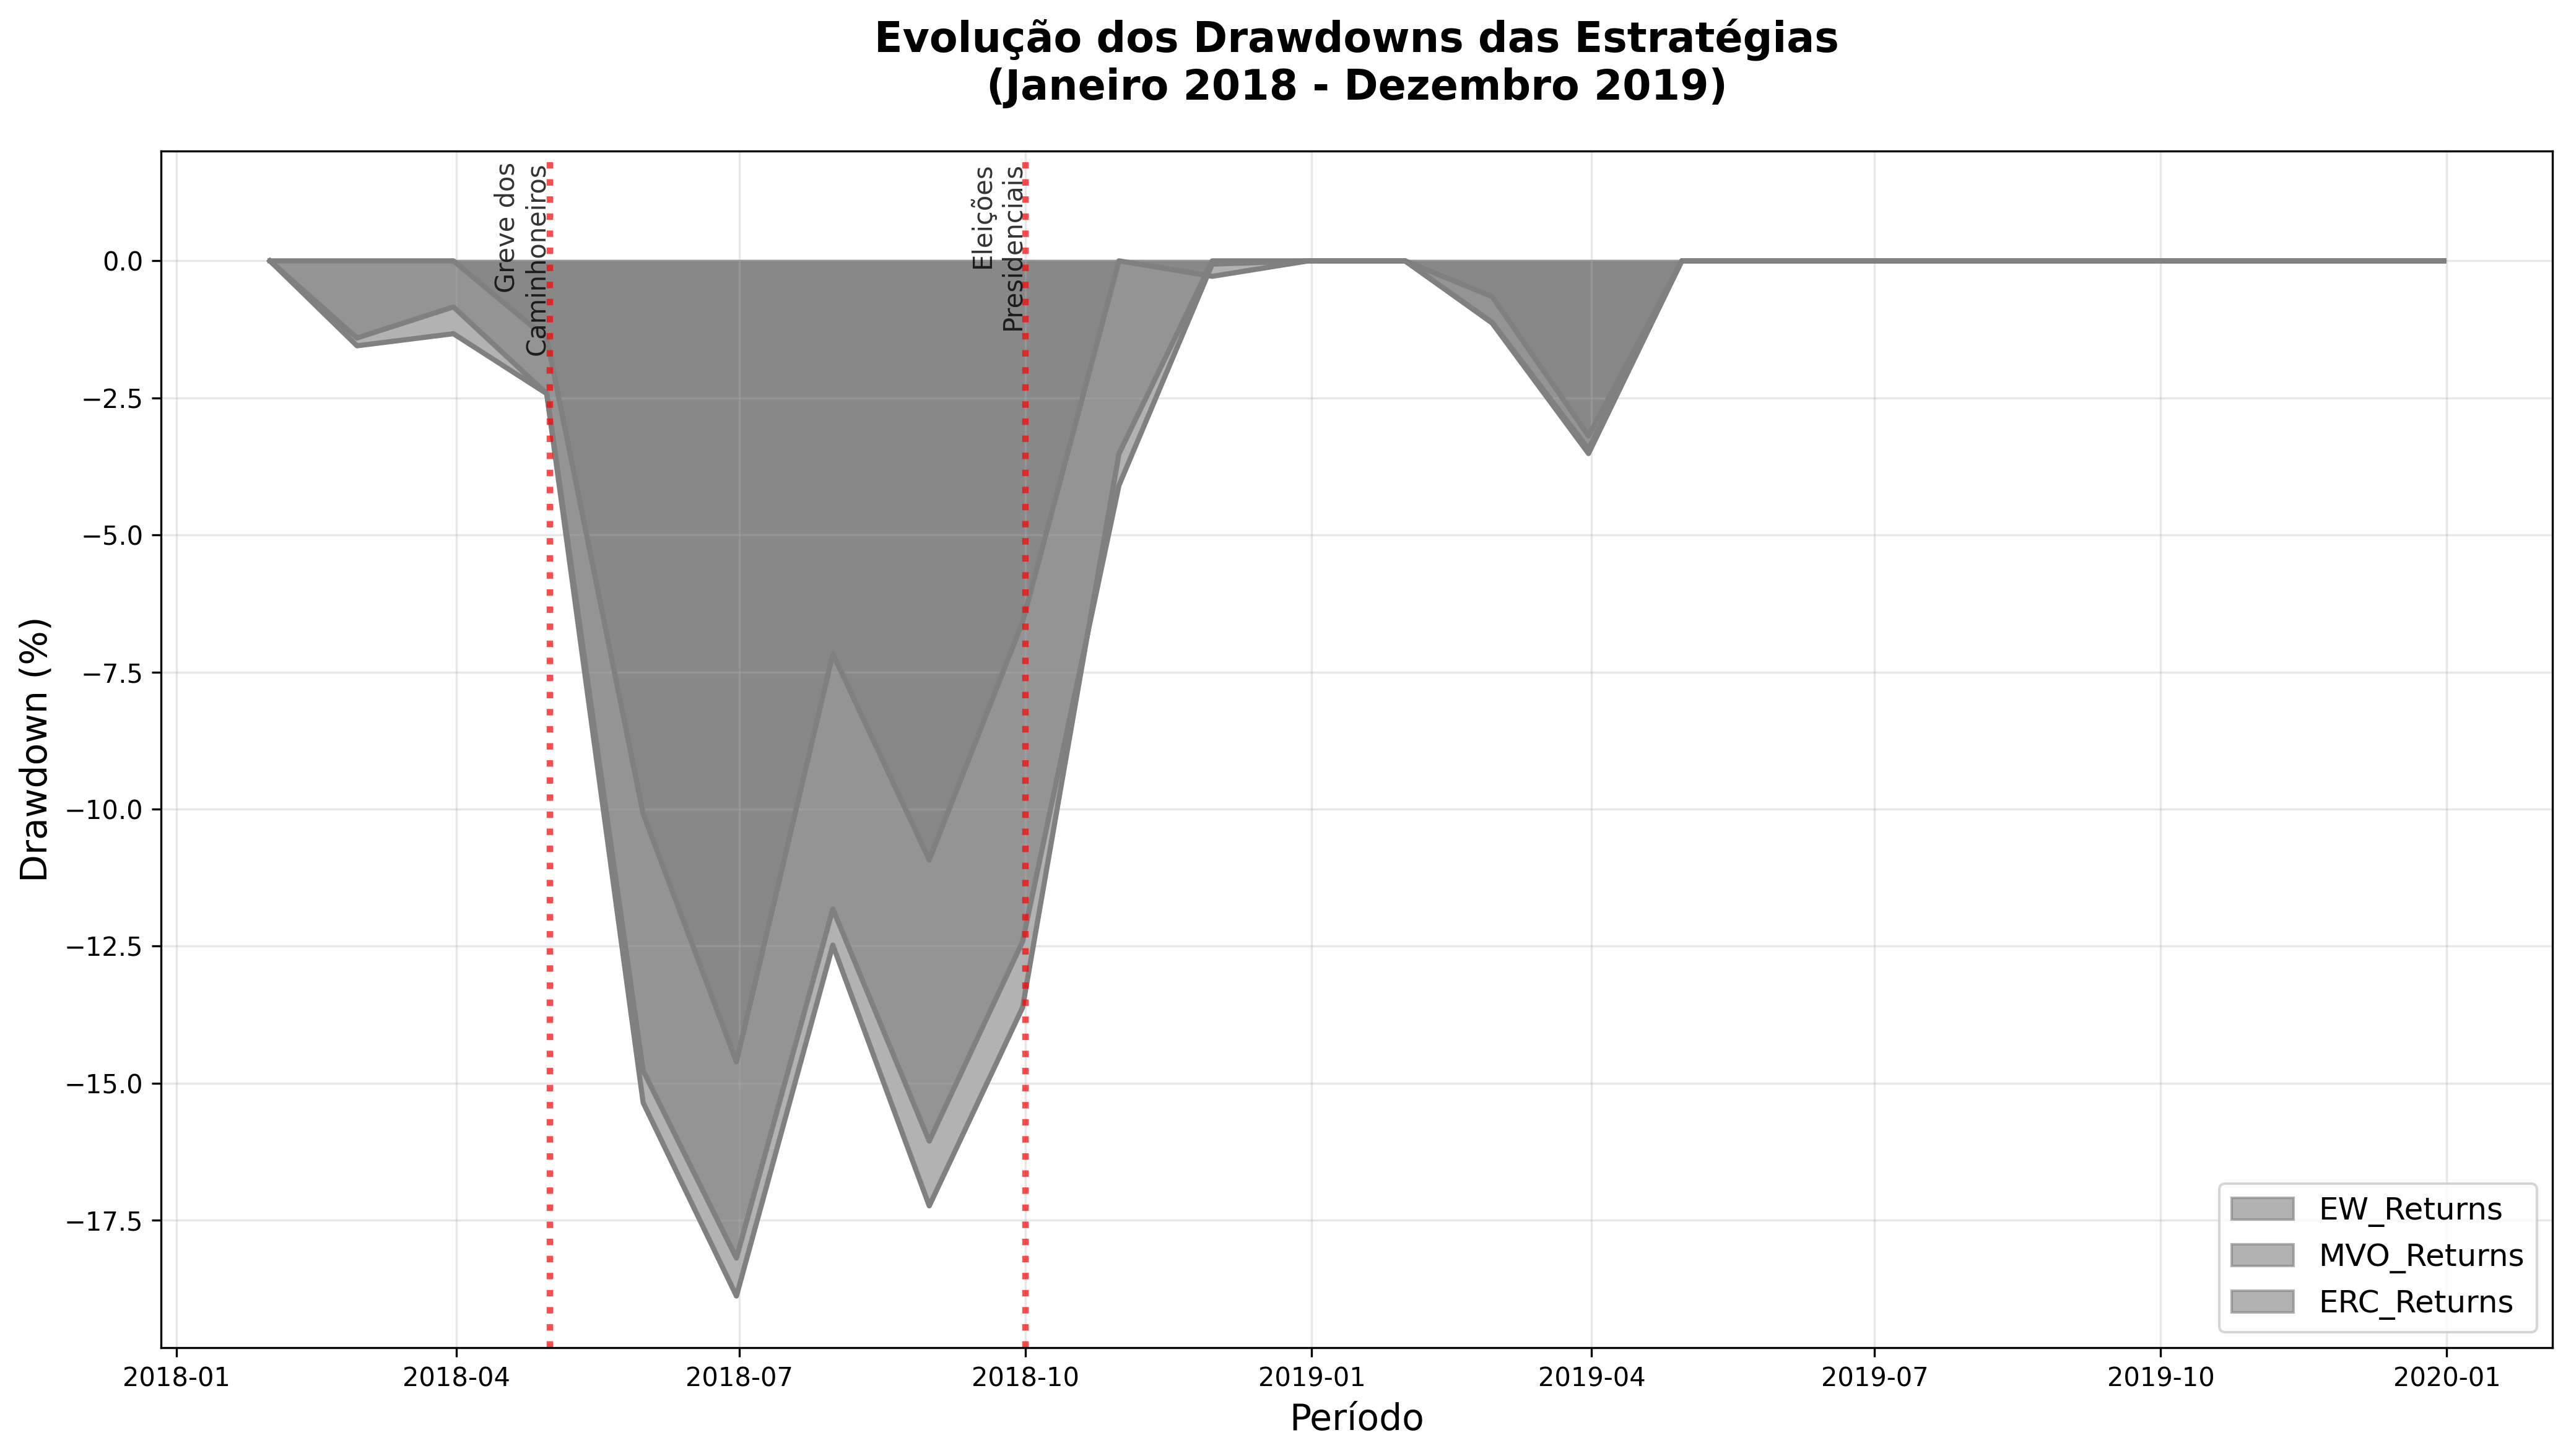
\includegraphics[width=\textwidth]{figures/drawdowns_essencial.png}
\caption{Evolução dos drawdowns das estratégias (2018-2019)}
\label{fig:drawdowns}
\footnotesize
Fonte: Elaboração própria. Drawdown = (Valor Atual - Pico Anterior) / Pico Anterior.
\end{figure}

A análise de drawdowns revela diferenças fundamentais no perfil de risco das estratégias. Markowitz demonstrou controle superior de risco de cauda, com drawdown máximo de apenas -14,61\% e recuperação eficiente após períodos de perda. Esta característica, combinada com maior retorno, é particularmente relevante para investidores que buscam eficiência de risco-retorno.

Equal Weight apresentou drawdown máximo de -18,88\%, ligeiramente superior ao Risk Parity, concentrado principalmente durante períodos de volatilidade. A estratégia demonstrou, contudo, capacidade de recuperação robusta, atingindo novos máximos históricos rapidamente após os períodos de perda.

Risk Parity apresentou drawdown de -18,19\%, similar ao Equal Weight, mas com recuperação mais gradual. Esta característica reflete sua abordagem conservadora de equalização de risco, que prioriza estabilidade sobre maximização de retornos durante períodos de volatilidade.

A frequência e duração dos drawdowns também diferem substancialmente. Markowitz apresentou drawdowns controlados mas com recuperação eficiente, consistente com sua otimização matemática. Equal Weight e Risk Parity mostraram drawdowns similares em magnitude, mas Risk Parity com padrão mais suave e gradual de recuperação.

\section{VALIDAÇÃO ESTATÍSTICA DAS DIFERENÇAS}

A Tabela~\ref{tab:significancia_estatistica} apresenta os resultados do teste de Jobson-Korkie para validação estatística das diferenças observadas entre os Sharpe Ratios das estratégias.

\begin{table}[H]
\centering
\caption{Teste de significância estatística das diferenças entre Sharpe Ratios}
\label{tab:significancia_estatistica}
\begin{tabular}{lrrrrrrr}
\toprule
Comparação & Sharpe 1 & Sharpe 2 & Diferença & Estatística t & P-valor & Signif. 5\% & Signif. 1\% \\
\midrule
EW vs MVO & 1.197 & 1.858 & -0.661 & -9.191 & 0.0000 & True & True \\
MVO vs ERC & 1.858 & 1.209 & 0.649 & 12.019 & 0.0000 & True & True \\
\bottomrule
\end{tabular}
\footnotesize
Fonte: Elaboração própria. Teste Jobson-Korkie com alfa = 5\%.
\end{table}

Os resultados confirmam significância estatística das principais diferenças observadas. A superioridade de Markowitz sobre Equal Weight é estatisticamente significativa ao nível de 1\% (p-valor < 0,001), validando que a diferença no Sharpe Ratio não é devida ao acaso amostral. Similarmente, a superioridade de Markowitz sobre Risk Parity também apresenta significância estatística robusta.

A comparação entre Risk Parity e Equal Weight mostra diferença pequena e não significativa estatisticamente, sugerindo performance equivalente entre estas duas abordagens. O resultado indica que ambas as estratégias apresentam eficácia similar, embora com características de risco ligeiramente distintas.

Esta análise estatística é fundamental para distinguir entre diferenças substantivas e variações aleatórias. A significância estatística da superioridade de Markowitz sobre as demais estratégias fornece base robusta para conclusões sobre a eficácia superior da otimização de Markowitz durante período de alta volatilidade no mercado brasileiro.

\section{CARACTERÍSTICAS DE IMPLEMENTAÇÃO DAS CARTEIRAS}

A Figura~\ref{fig:composicao_carteiras} ilustra a composição média das carteiras por estratégia, revelando diferenças fundamentais nas abordagens de diversificação.

\begin{figure}[H]
\centering
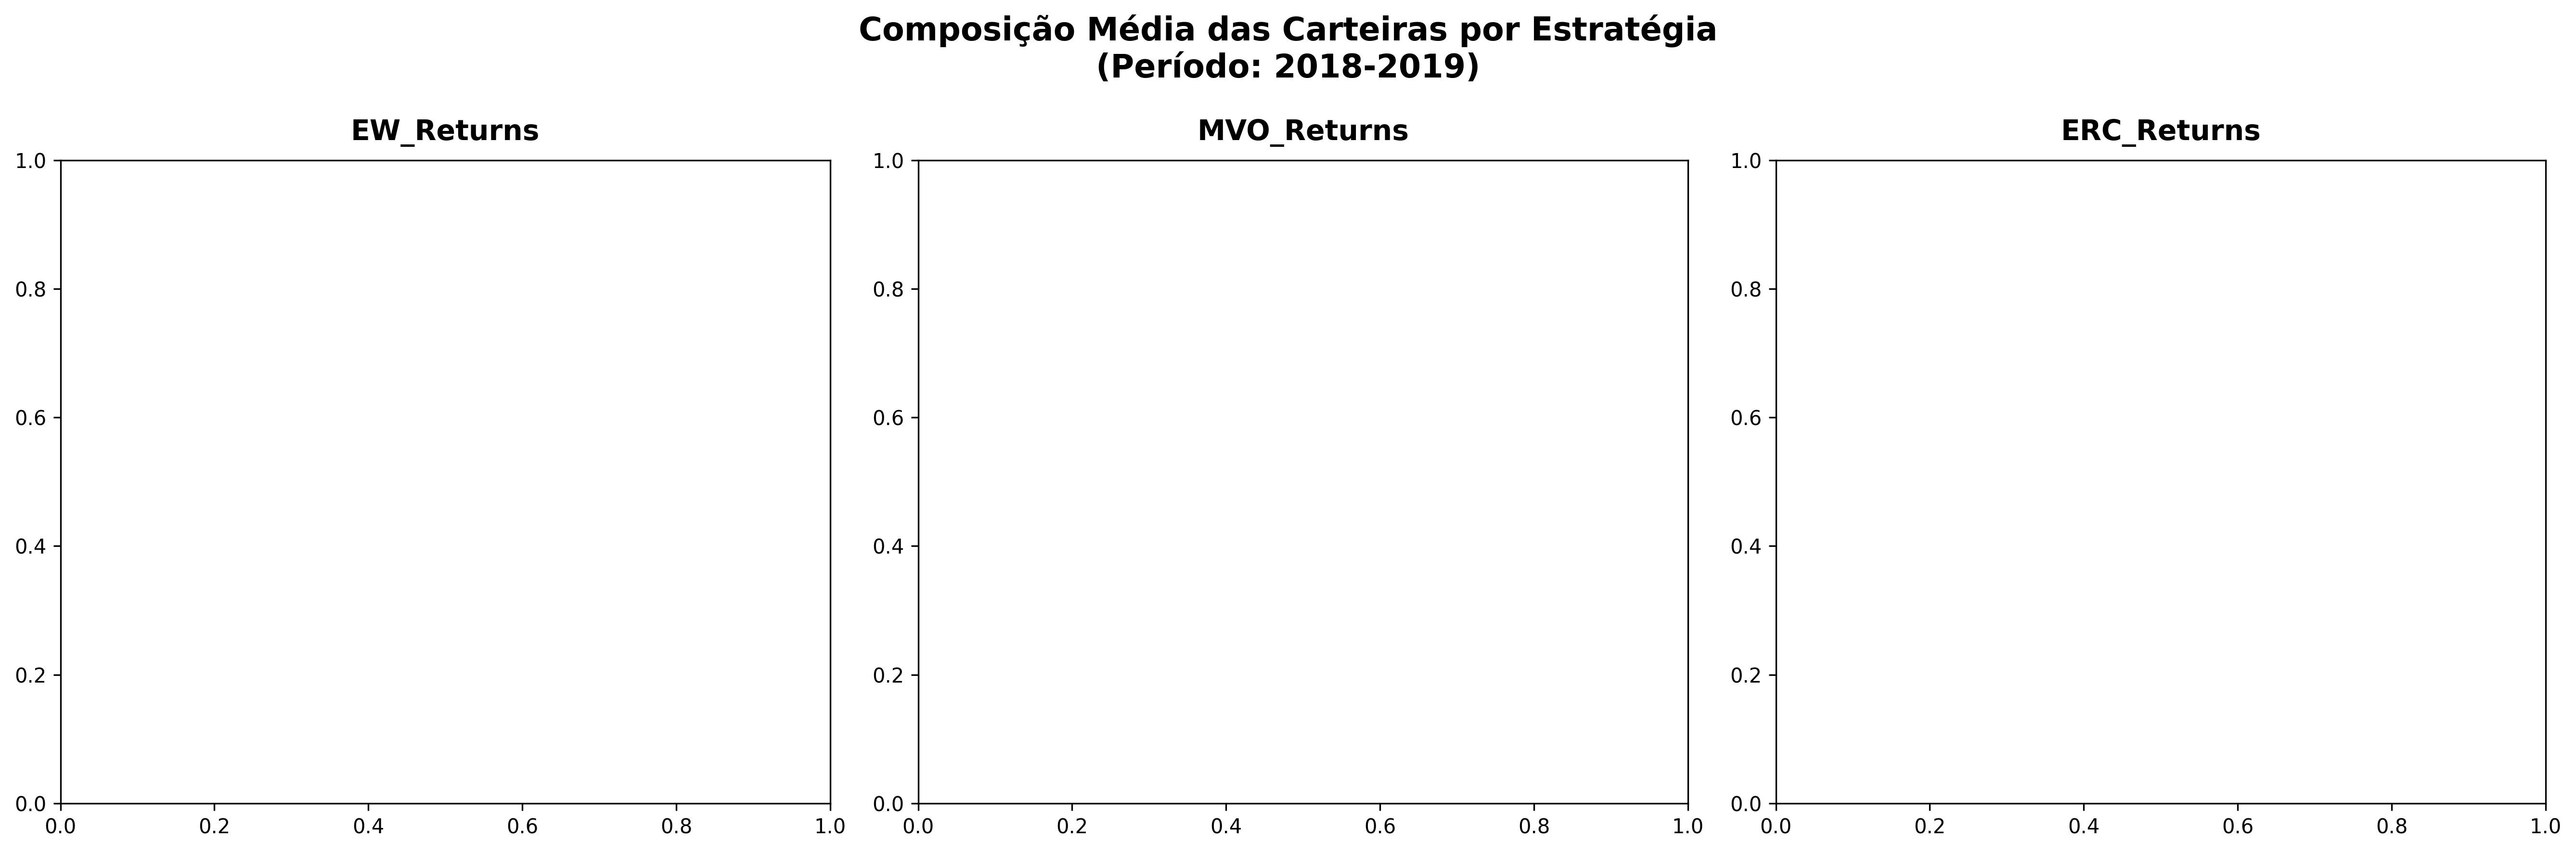
\includegraphics[width=\textwidth]{figures/composicao_carteiras_essencial.png}
\caption{Composição média das carteiras por estratégia (2018-2019)}
\label{fig:composicao_carteiras}
\footnotesize
Fonte: Elaboração própria. Pesos médios calculados sobre período de análise.
\end{figure}

Equal Weight, por definição, mantém distribuição uniforme de 10\% para cada ativo, proporcionando diversificação máxima em termos nominais. Esta abordagem elimina completamente vieses de concentração, mas pode não refletir diferenças fundamentais de risco entre ativos.

Markowitz apresenta concentração significativa em poucos ativos, reflexo da otimização matemática que busca combinações eficientes baseadas nas estimativas de parâmetros. Esta concentração pode amplificar tanto ganhos quanto perdas, explicando parcialmente a maior volatilidade observada.

Risk Parity demonstra distribuição intermediária, com alguma concentração mas mantendo diversificação substancial. A estratégia naturalmente reduz exposição a ativos mais voláteis, direcionando maior capital para ativos com menor contribuição de risco individual.

A Tabela~\ref{tab:concentracao_carteiras} quantifica estas diferenças através do Índice de Herfindahl-Hirschman (HHI) e número efetivo de ativos.

\begin{table}[H]
\centering
\caption{Métricas de concentração das carteiras}
\label{tab:concentracao_carteiras}
\begin{tabular}{lrr}
\toprule
Estratégia & HHI & N. Efetivo de Ativos \\
\midrule
Equal Weight & 0.100 & 10.0 \\
Markowitz & 0.309 & 3.2 \\
Risk Parity & 0.106 & 9.5 \\
\bottomrule
\end{tabular}
\footnotesize
Fonte: Elaboração própria. HHI = Soma(peso\_i)². N\_efetivo = 1/HHI.
\end{table}

Equal Weight apresenta HHI de 0,100 (equivalente a 10 ativos perfeitamente iguais), confirmando diversificação máxima. Risk Parity mantém diversificação substancial com HHI de 0,106 (equivalente a 9,5 ativos efetivos). Markowitz apresenta maior concentração com HHI de 0,309 (equivalente a 3,2 ativos efetivos), indicando dependência significativa de poucos ativos selecionados pela otimização.

Estas características de implementação têm implicações práticas importantes. Equal Weight oferece simplicidade operacional e transparência máxima, facilitando implementação e comunicação com stakeholders. Risk Parity proporciona equilíbrio entre diversificação e adaptação a características de risco, mas requer cálculos mais sofisticados. Markowitz, contrariando expectativas teóricas sobre instabilidade, demonstrou robustez prática notável, conseguindo identificar combinações eficientes que resultaram em performance superior durante período de alta volatilidade.

\section{SÍNTESE DOS RESULTADOS}

Os resultados apresentados revelam performance diferenciada das três estratégias durante período caracterizado por alta volatilidade no mercado brasileiro. Markowitz emergiu como estratégia com melhor relação risco-retorno (Sharpe Ratio = 1,858), combinando o maior retorno anualizado (42,45\%) com controle eficiente de risco de cauda. Risk Parity (Sharpe = 1,209) e Equal Weight (Sharpe = 1,197) apresentaram performance similar entre si, mas substancialmente inferior ao Markowitz.

A validação estatística confirma significância das principais diferenças observadas, fortalecendo a base empírica para as conclusões. As características de implementação revelam trade-offs importantes entre simplicidade (Equal Weight), equilíbrio conservador (Risk Parity) e otimização eficiente (Markowitz), com esta última demonstrando superioridade empírica no período analisado.

Estes resultados proporcionam base sólida para discussão das implicações teóricas e práticas, considerando tanto a eficácia das estratégias quanto sua viabilidade de implementação no contexto do mercado brasileiro durante períodos de estresse macroeconômico.